% Created 2023-02-02 Thu 13:24
% Intended LaTeX compiler: lualatex
\documentclass[11pt]{article}
\usepackage{graphicx}
\usepackage{longtable}
\usepackage{wrapfig}
\usepackage{rotating}
\usepackage[normalem]{ulem}
\usepackage{amsmath}
\usepackage{amssymb}
\usepackage{capt-of}
\usepackage{hyperref}
\usepackage{minted}
\usepackage{physics}
\usepackage[margin=0.5in]{geometry}
\author{David Lewis}
\date{\today}
\title{Lecture 8 notes}
\hypersetup{
 pdfauthor={David Lewis},
 pdftitle={Lecture 8 notes},
 pdfkeywords={},
 pdfsubject={},
 pdfcreator={Emacs 28.2 (Org mode 9.6)}, 
 pdflang={English}}
\begin{document}

\maketitle

\section*{Guest lecturer: Abhiram Natarajan}
\label{sec:org7240c16}
\begin{quote}
Methods in Algebraic Geometry towards Data Science Applications
\end{quote}
\subsection*{Intro}
\label{sec:org70a763f}
\begin{itemize}
\item Algebraic geometry deals with  non-linar objects(Polynomials)
\item more computationally expensive
\end{itemize}
\subsubsection*{algebraic geometry}
\label{sec:org594515c}
\begin{itemize}
\item study the 0s of polynomials
\item \(Z(f):=\{X\) such that \(f(X) = 0\}\)
\end{itemize}
\begin{center}
\begin{tabular}{ll}
Polynomial & Zeros\\
\hline
f(x) = x - 7 & Z(f) = $\backslash${7$\backslash$}\\
\(f_1(x,y) = y-x\) & line through the origin\\
\end{tabular}
\end{center}
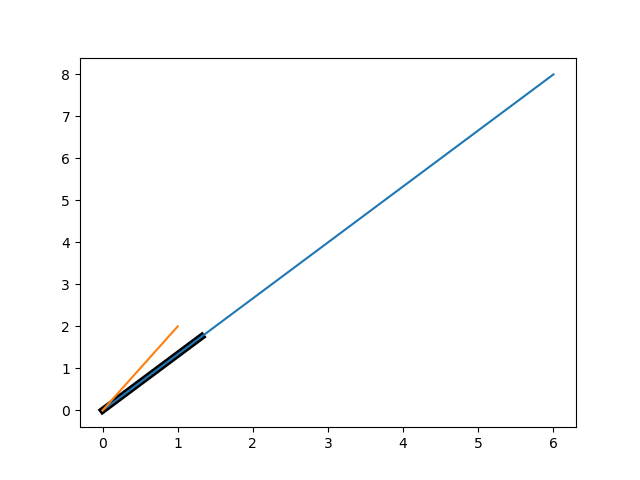
\includegraphics[width=\textheight,height=\textwidth,keepaspectratio]{/home/david/Documents/Planner/Intelligent_Data_Design/lec8/images/1.png}
\begin{itemize}
\item Question
\label{sec:org7db365e}
\begin{itemize}
\item Given a set of polynomials, find all the common zeros
\item Gaussien elimination is used in the linear case
\end{itemize}
\end{itemize}

\subsection*{Grobner Bases}
\label{sec:org072961a}
\begin{itemize}
\item 2 equations, two variables
\end{itemize}
\subsubsection*{Gausiien alimination}
\label{sec:org47b6ef0}
\begin{itemize}
\item Elimiminate leading term for every pair of linear equations
\item Continue until you reach and equation with just one variable
\item Solve system with back substitution
\end{itemize}
\subsubsection*{Two polynomials}
\label{sec:orgc2e3c98}
\begin{itemize}
\item \(x^2y^3 - 4 = 0\)
\item \(x^3y^2 - 2 = 0\)
\item multiply first polynomial by x, second by y
\item \(x^3y^3 - 4x = 0\)
\item \(x^3y^3 - 4y = 0\)
\item subtract the equations
\item \(y = 2x\)
\item plug into original polynomial
\item \(x = 1\)
\end{itemize}
\subsubsection*{generalized gaussian}
\label{sec:orga09129c}
\begin{itemize}
\item modified gaussian works in the non-linear case
\item S-polynomial of f and g is S(f,g)
\item compute every S polynomial of every possible pair of polynomials until system
can be solved
\item set of all S-polynomials is called a Grobner Basis
\end{itemize}
\subsubsection*{Buchberger's Algorithm for Grobner Basis}
\label{sec:orgddd351b}
\begin{itemize}
\item iterate over every pair of polynomials in S
\item compute S(f,G) and add it to S'
\item repeat until S is solvable
\end{itemize}
\subsubsection*{Geometrity of gaussian elimination}
\label{sec:org64df37f}
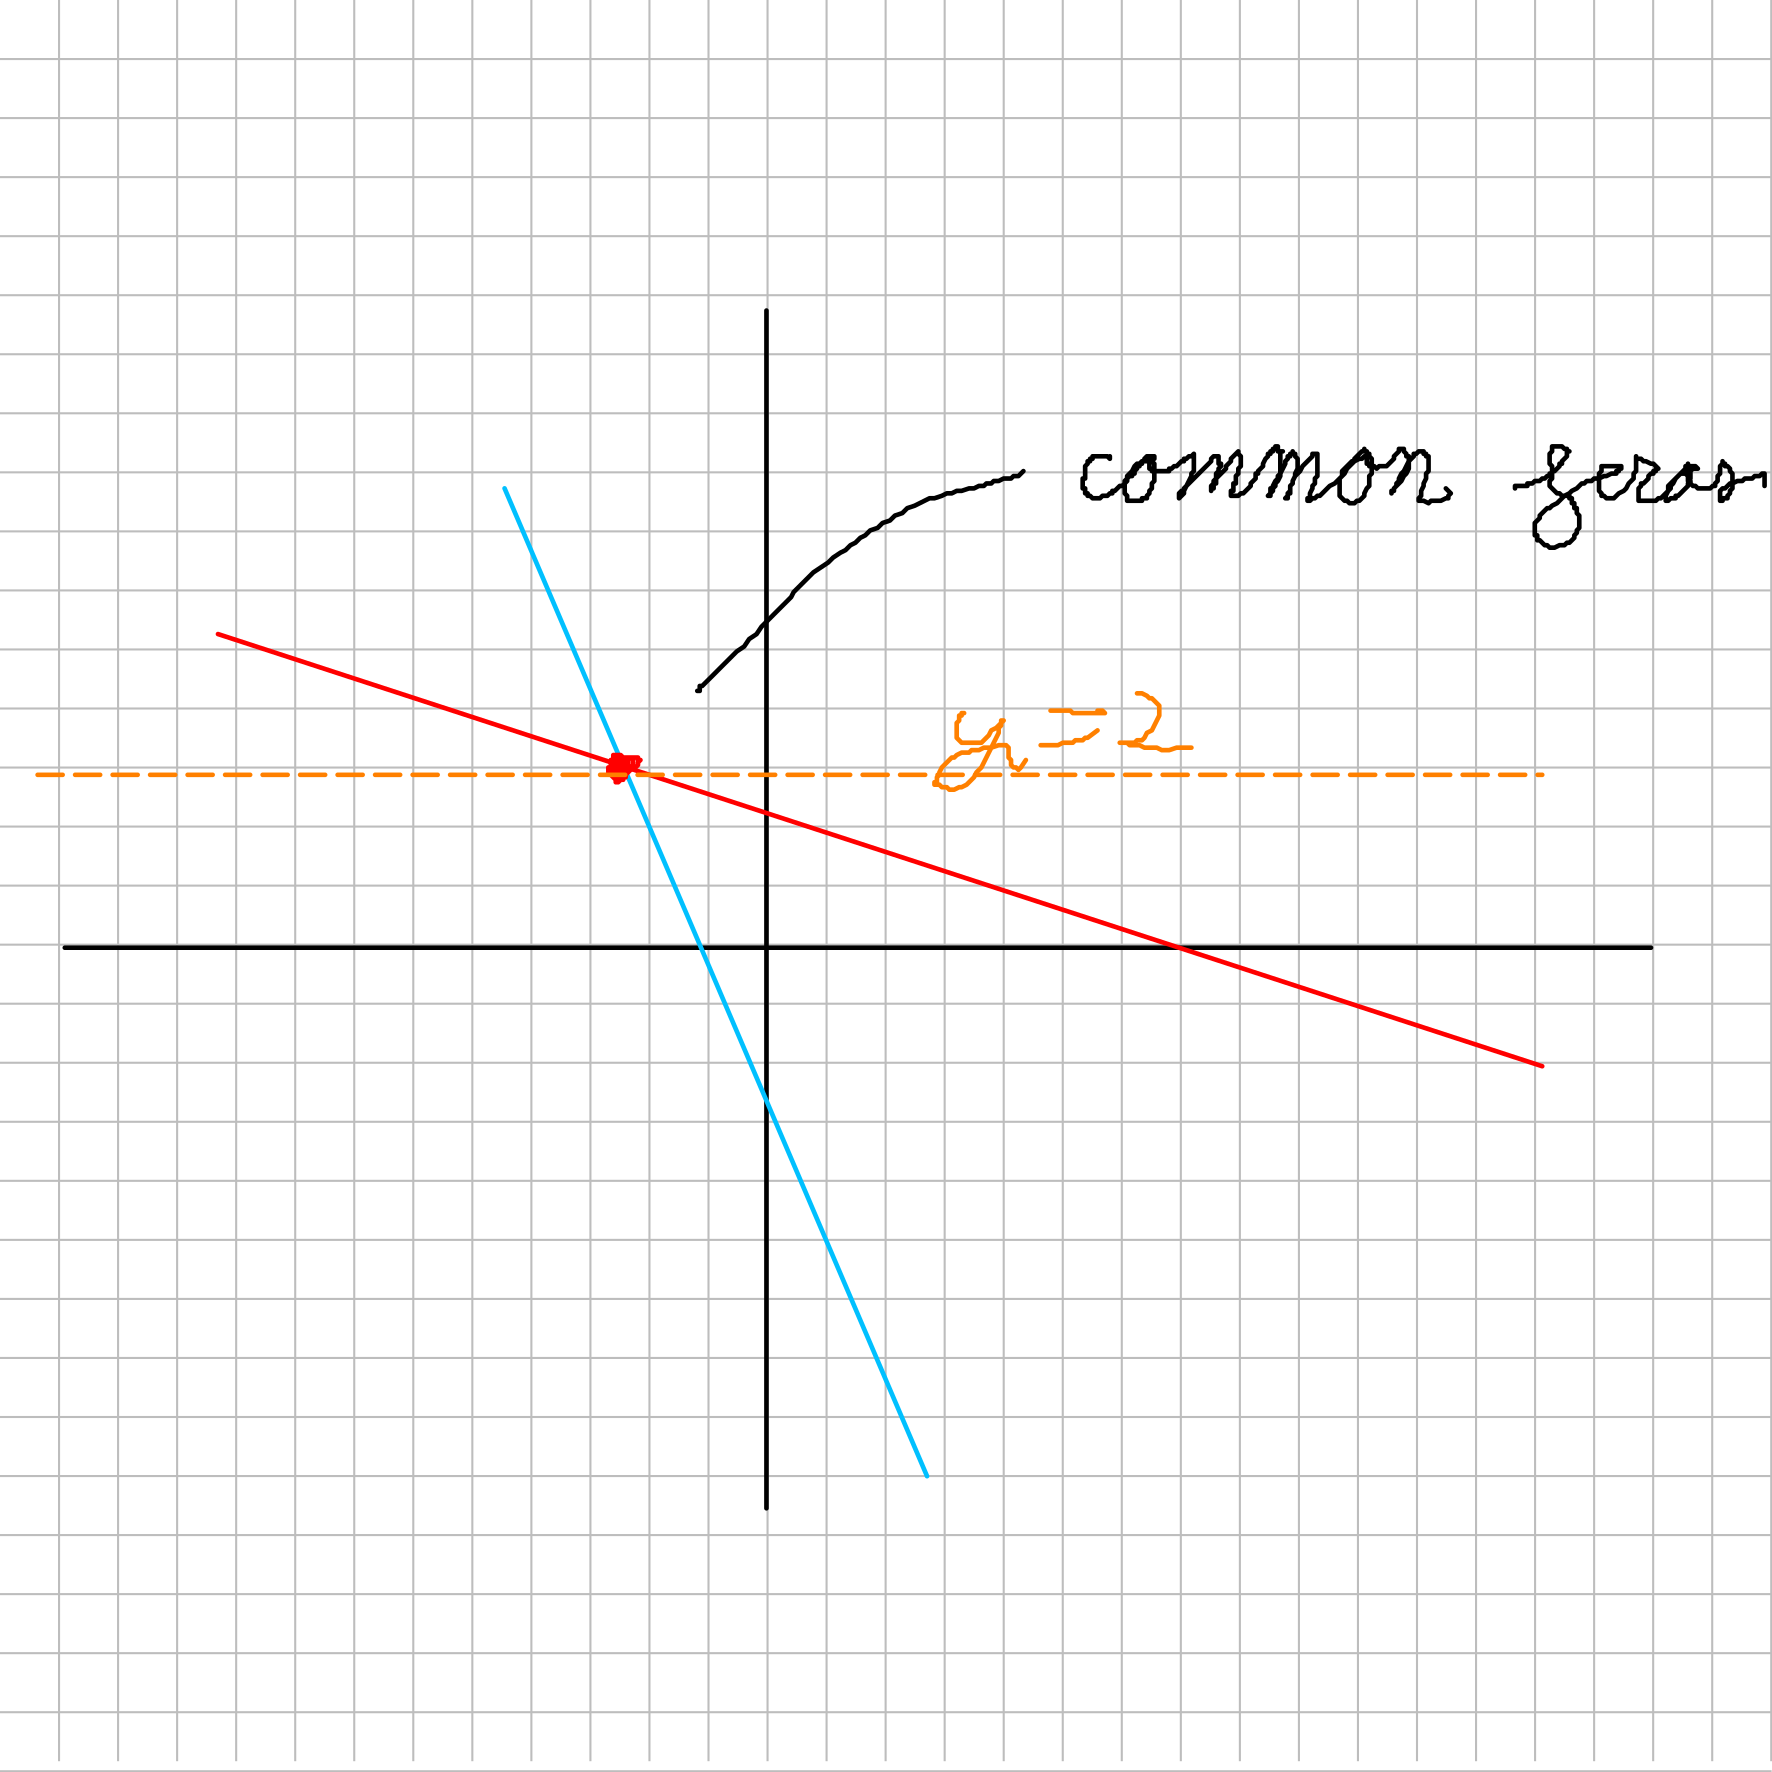
\includegraphics[width=\textheight,height=\textwidth,keepaspectratio]{/home/david/Documents/Planner/Intelligent_Data_Design/lec8/images/geometry.png}
\subsubsection*{Geometry of Grobner Basis}
\label{sec:org412163e}
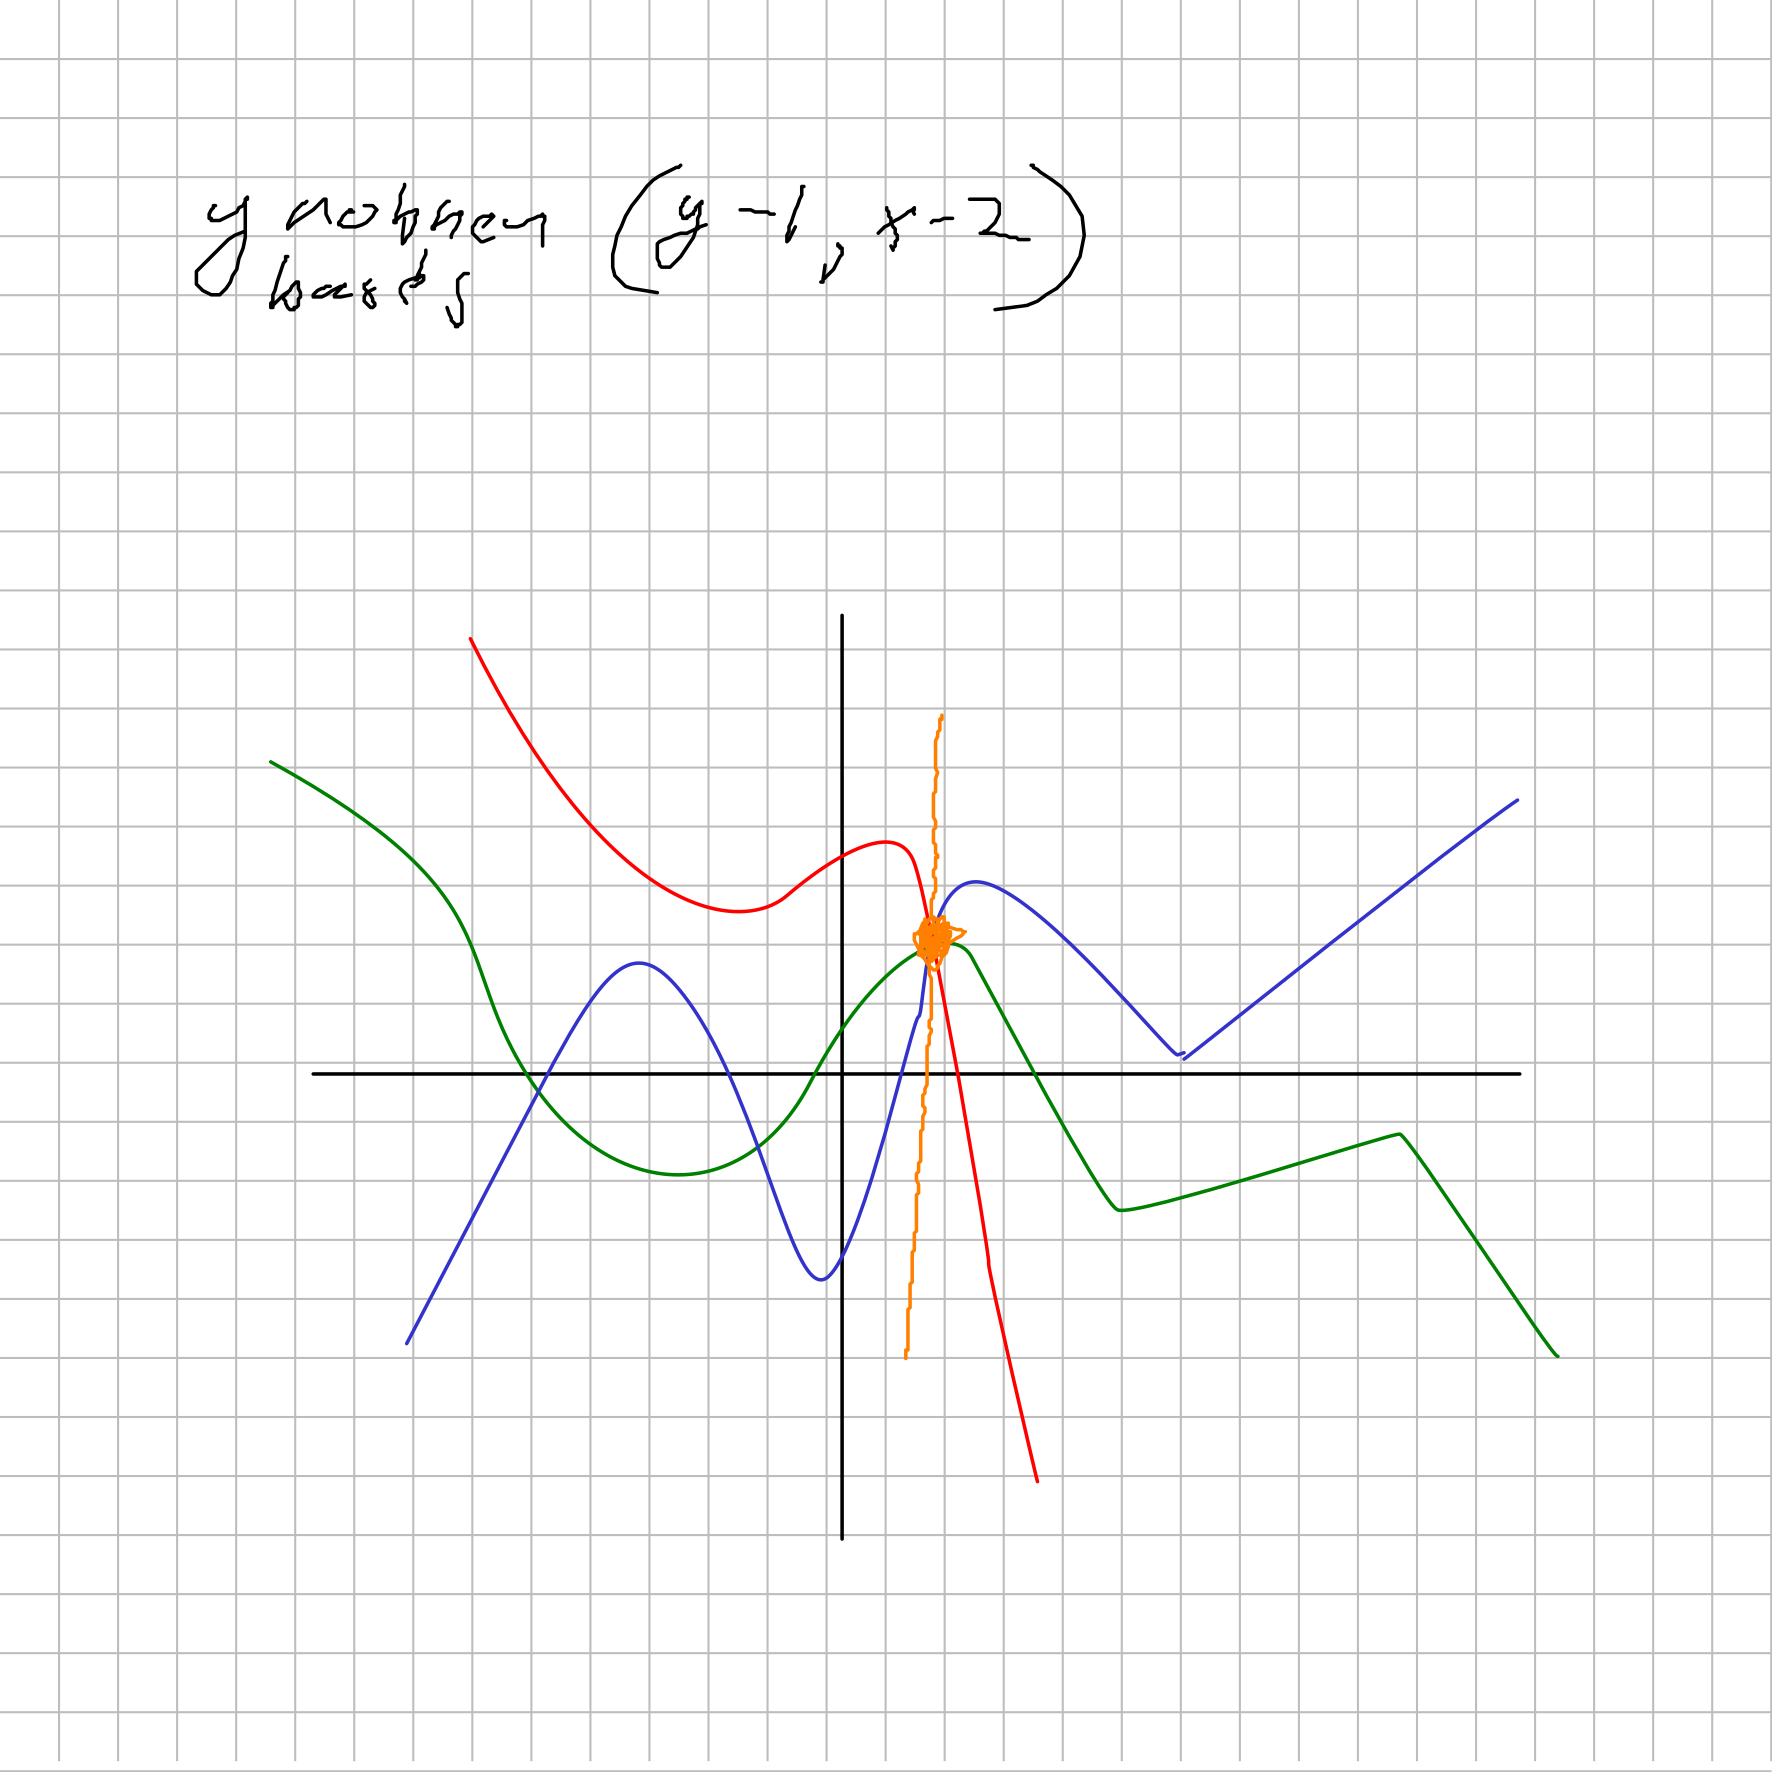
\includegraphics[width=\textheight,height=\textwidth,keepaspectratio]{/home/david/Documents/Planner/Intelligent_Data_Design/lec8/images/grobner.png}

\subsection*{Applications of Grobner Bases}
\label{sec:org95d11c5}
\begin{itemize}
\item S is not solvable if and only if the grobner basis contains a constant
polynomial
\item This is show gemetrically by intersections in the zero polynomials
\end{itemize}
\subsubsection*{Sudoku}
\label{sec:orgfaab531}
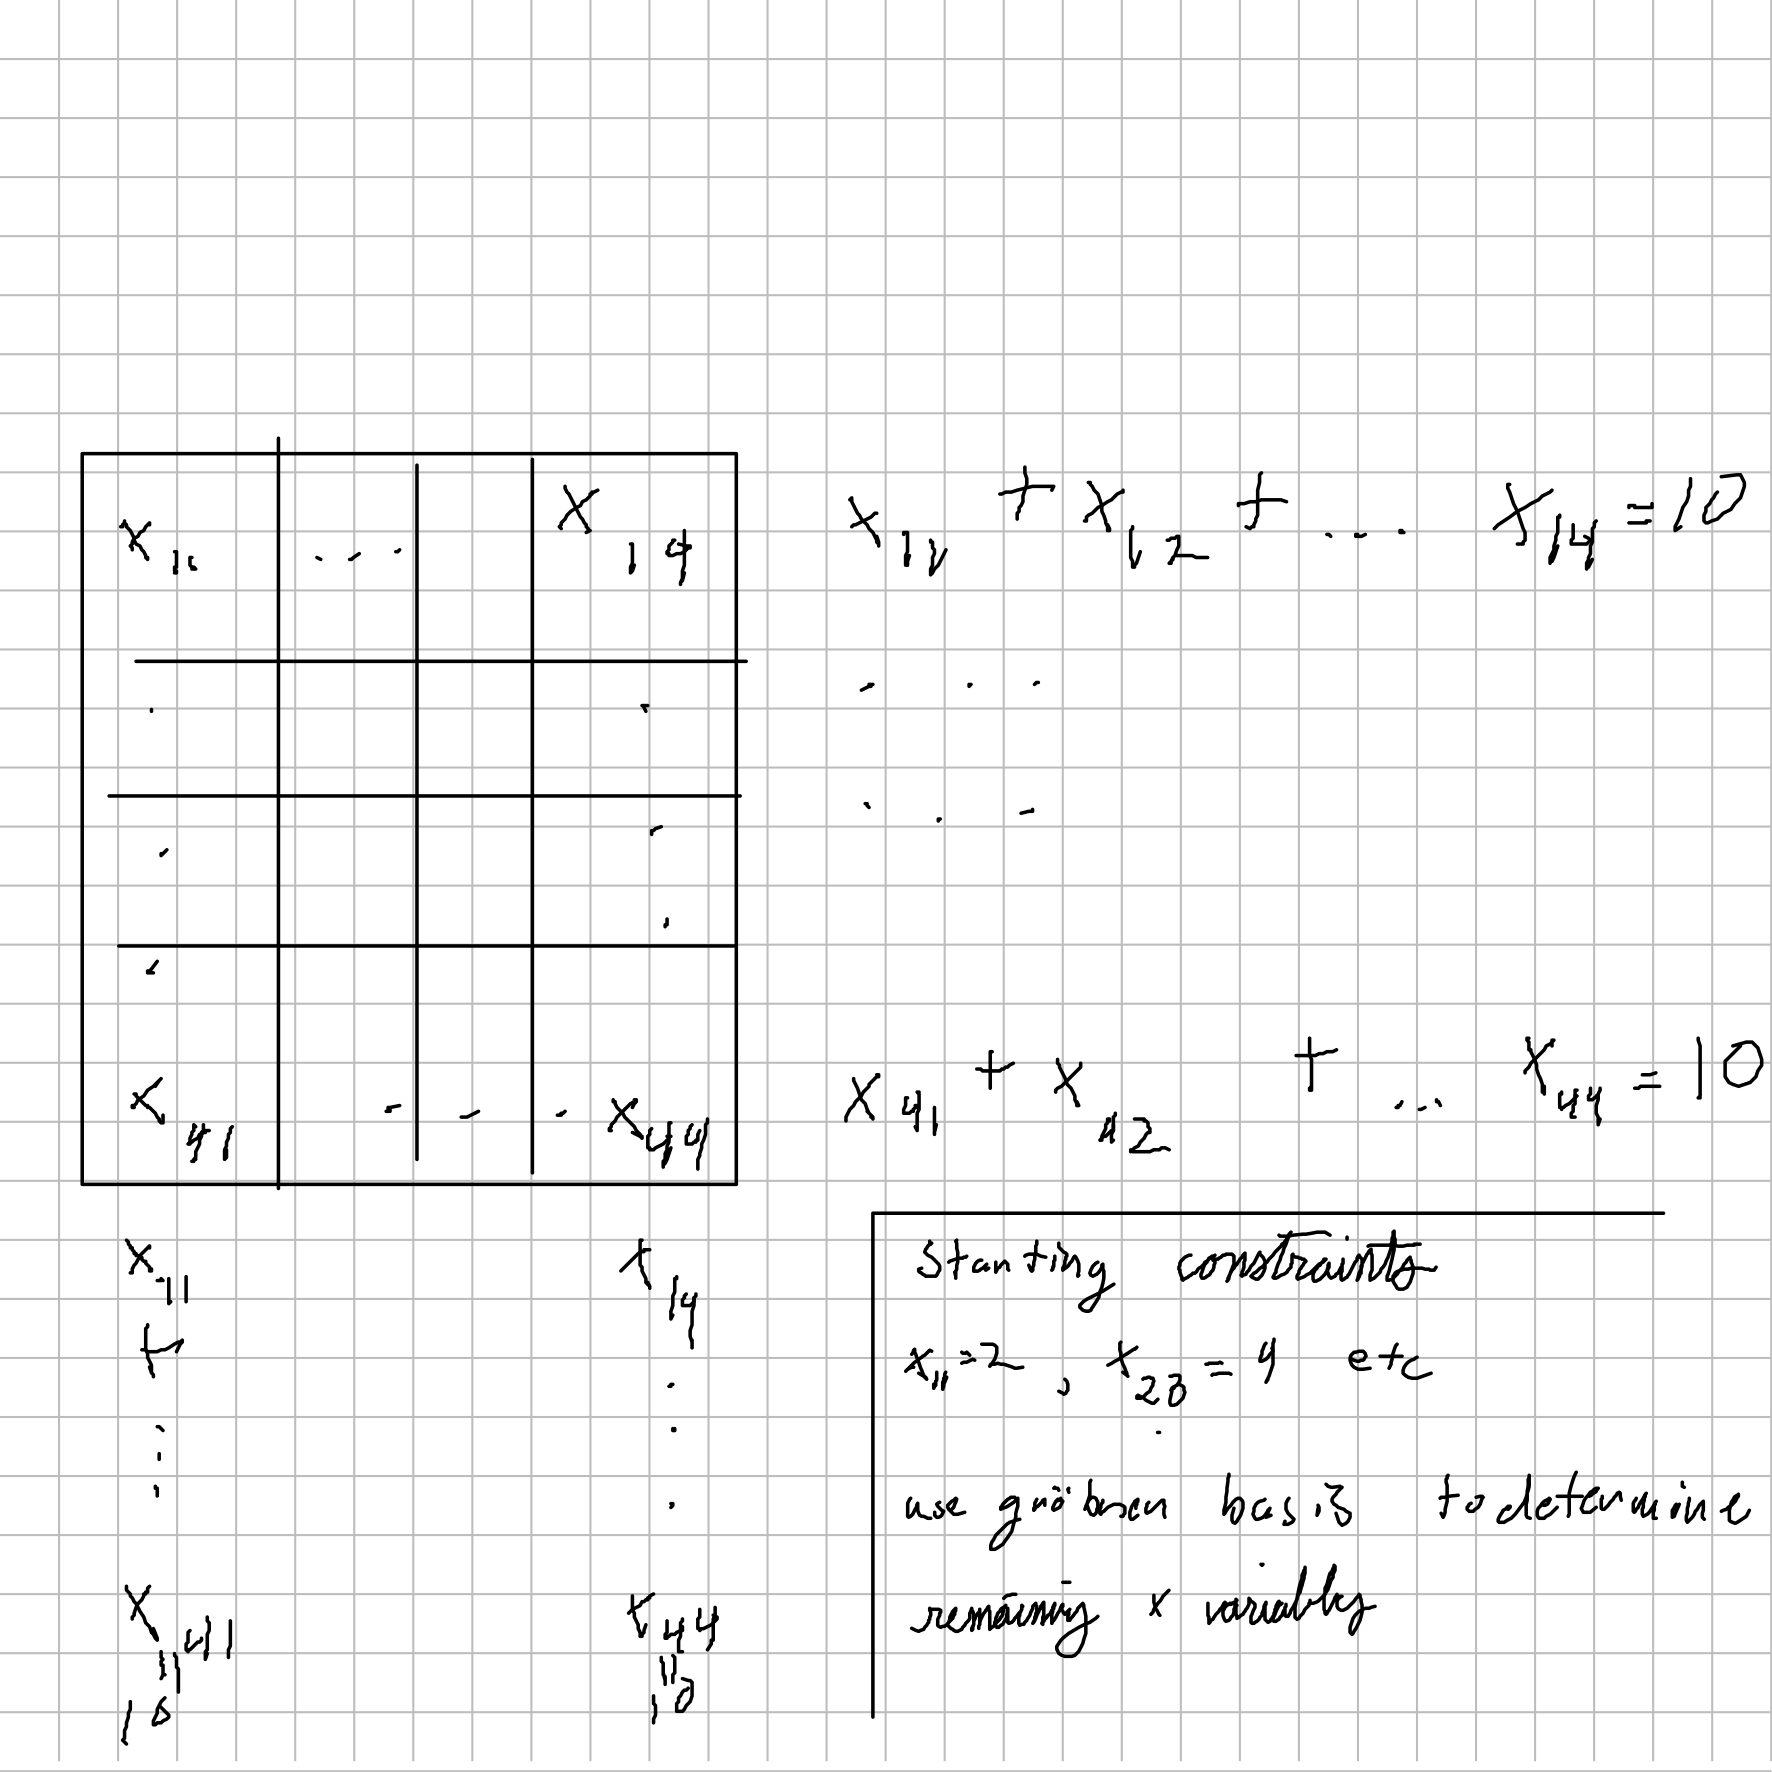
\includegraphics[width=\textheight,height=\textwidth,keepaspectratio]{/home/david/Documents/Planner/Intelligent_Data_Design/lec8/images/sudoku.png}
\begin{itemize}
\item Must contain all numbers 1,4 exactly once
\item All columns and rows must add up to 10
\item Use grobner basis to reduce polynomial to solvable state
\end{itemize}
\subsection*{Conclusion}
\label{sec:orgc0801a3}
\begin{itemize}
\item Grobner bases are a very power notion
\item many applications (automated geometry theorem, robotics, sudoku, etc)
\item critical insight into any system of polynomials
\item lots of software can compute grobner bases
\end{itemize}
\end{document}
